\subsubsection{Hardware Security Analysis: Timing-flow Analysis}

The timing-flow analysis is described in Section~\ref{sec:client-timingflow};
this section focuses on its evaluation (Figure~\ref{fig:eval-timingflow}).

\begin{figure}[tp]
    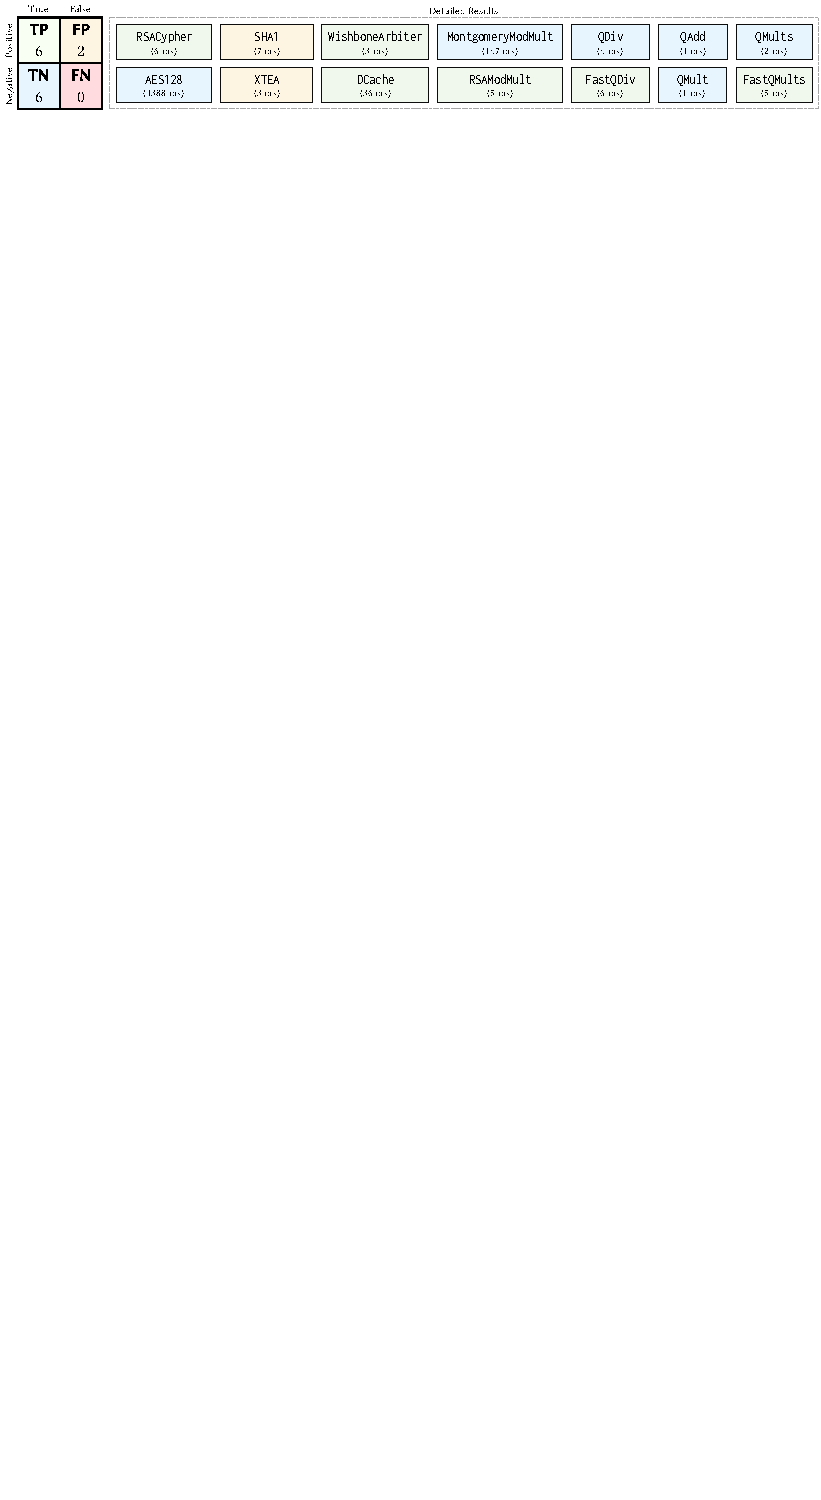
\includegraphics[clip,trim=0 23.5cm 0 0]{figures/timingflow-eval}
    \caption{Evaluation of timing-flow analysis (recall: 100\%, precision: 75\%), a hardware security client built on top of \tia; analysis times are shown in parentheses.}\label{fig:eval-timingflow}
\end{figure}

\paragraph{Benchmarks}

Our timing-flow analysis is inspired by a survey of hardware information-flow tracking~\cite{hu_hardware_2022}, which describes information leaks through timing flows and summarizes representative hardware designs for which prior work~\cite{ardeshiricham_clepsydra_2017,qin_formal_2020,alatoun_efficient_2022} has established the presence or absence of timing flows.
We select all such designs available to us as benchmarks to evaluate our timing-flow analysis.
These designs, shown in the dashed box in the right part of Figure~\ref{fig:eval-timingflow}, include cryptographic components from TrustHub~\cite{salmani_design_2013,shakya_benchmarking_2017} (\texttt{RSACypher}~\cite{rsa-cypher} and \texttt{AES128}~\cite{aes128}) and OpenCores~\cite{opencores} (\texttt{SHA1}~\cite{sha1} and \texttt{XTEA}~\cite{xtea}), a round-robin-based Wishbone arbiter (\texttt{WishboneArbiter}~\cite{wishbone-arbiter}), a data cache (\texttt{DCache} described by~\cite{qin_formal_2020}), modular multipliers (\texttt{MontgomeryModMult}~\cite{montgomery-modmult} and \texttt{RSAModMult}~\cite{rsa-modmult}), and fixed-point arithmetic units~\cite{fixed-point-math} and their variants described by~\cite{qin_formal_2020,ardeshiricham_clepsydra_2017}.

\paragraph{Understanding the Results}


The left part of Figure~\ref{fig:eval-timingflow} summarizes the overall results of timing-flow analysis, while the right part details the results for each benchmark, with colors indicating the classification.
There are 6 true positives (TPs, in green), where our analysis correctly identifies timing-flow information leaks in vulnerable designs, and 6 true negatives (TNs, in blue), where it correctly identifies secure designs without timing flows as secure.
There are no false negatives (FNs, in red), where our analysis fails to detect a true timing-flow information leak, yielding a recall of $\mathit{recall} = \mathit{TP}/(\mathit{TP}+\mathit{FN}) = 100\%$.
There are two false positives (FPs, in yellow), where our analysis reports a timing-flow information leak in a secure design, yielding a precision of $\mathit{precision} = \mathit{TP}/(\mathit{TP}+\mathit{FP}) = 75\%$.
The two false positives occur in \texttt{SHA1} and \texttt{XTEA} and are caused by \tia's path insensitivity.
Specifically, path insensitivity allows spurious temporal influences from the private source to the public sink that indicate timing flows, even though not all of these influences can occur under the actual combination of multiplexer conditions.

As indicated by the analysis times in parentheses under the benchmark names in Figure~\ref{fig:eval-timingflow}, our timing-flow analysis is also efficient, taking an average analysis time of 115.3 milliseconds across the benchmarks, including the time spent by the underlying \tia.
This efficiency stems from both the efficiency of \tia and the lightweight reuse of its computed temporal influence information: the client analysis only queries \tia's results to identify multiple temporal influences that indicate timing flows, as described in Section~\ref{sec:client-timingflow}, and therefore incurs little additional computational overhead.
The \texttt{AES128} benchmark takes more than one second to analyze, substantially longer than the other benchmarks combined, because it is much larger than the other benchmarks combined (98.4K LoC vs. 1.6K LoC in pre-elaborated Firrtl~\cite{izraelevitz_reusability_2017}).
